\documentclass[tikz,border= 1cm]{standalone}
\usetikzlibrary{calc}
\begin{document}
	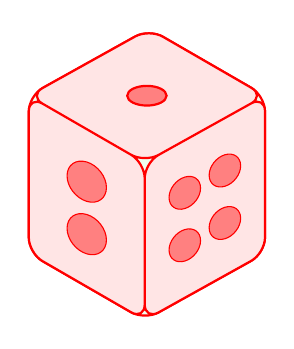
\begin{tikzpicture}[rounded corners=2mm]
		\def\a{2}
		\path(0,0)coordinate(A)++(-30:0.85*\a)coordinate(B)(1.5*\a,0)coordinate(C)($(A)+(C)-(B)$)coordinate(D);
		\path[shift={(0,\a)}](0,0)coordinate(A')++(-30:0.85*\a)coordinate(B')(1.5*\a,0)coordinate(C')($(A')+(C')-(B')$)coordinate(D');
		\fill[green!20!white!30,draw=red,thick](A)--(A')--(D')--(C')--(C)--(B)--cycle;
		\draw[fill=red!10,draw=red,thick](B)--(C)--(C')--(B')--cycle (A')--(B')--(C')--(D')--cycle (A)--(A')--(B')--(B)--cycle;
		%%%nút 1
		\fill[yscale=0.5,draw=red,fill=red!50,thick]($(A')!0.5!(C')$)circle(0.125*\a);
		%%%nút 2
		\path($(A')!0.5!(B')$)coordinate(M') ($(A)!0.5!(B)$)coordinate(M);
		\fill[yslant=-0.3,draw=red,fill=red!50]($(M)!1/3!(M')$) circle (0.125*\a)
		($(M)!2/3!(M')$) circle (0.125*\a);
		%%%nút 3
		\path($(B')!1/3!(C')$)
		coordinate(N')($(B)!1/3!(C)$)coordinate(N)($(B')!2/3!(C')$)coordinate(P')($(B)!2/3!(C)$)coordinate(P);
		\fill[yslant=0.3,draw=red,fill=red!50]($(N)!1/3!(N')$)circle(0.1*\a)($(N)!2/3!(N')$)circle(0.1*\a)($(P)!1/3!(P')$)circle(0.1*\a)($(P)!2/3!(P')$)circle(0.1*\a);
	\end{tikzpicture}
\end{document}